%*
%* Seven Kingdoms: Ancient Adversaries
%*
%* Copyright 1997,1998 Enlight Software Ltd.
%* Copyright 2018 Timothy Rink
%*
%* This program is free software: you can redistribute it and/or modify
%* it under the terms of the GNU General Public License as published by
%* the Free Software Foundation, either version 2 of the License, or
%* (at your option) any later version.
%*
%* This program is distributed in the hope that it will be useful,
%* but WITHOUT ANY WARRANTY; without even the implied warranty of
%* MERCHANTABILITY or FITNESS FOR A PARTICULAR PURPOSE.  See the
%* GNU General Public License for more details.
%*
%* You should have received a copy of the GNU General Public License
%* along with this program.  If not, see <http://www.gnu.org/licenses/>.
%*
%*

\chapter[Fryhtans and Their Ways]{\textsf{{\Huge F}RYHTANS AND {\Huge T}HEIR {\Huge W}AYS}}

\section{\textsf{Fryhtan Lairs}}

\index{Fryhtans!lairs}

\begin{center}
    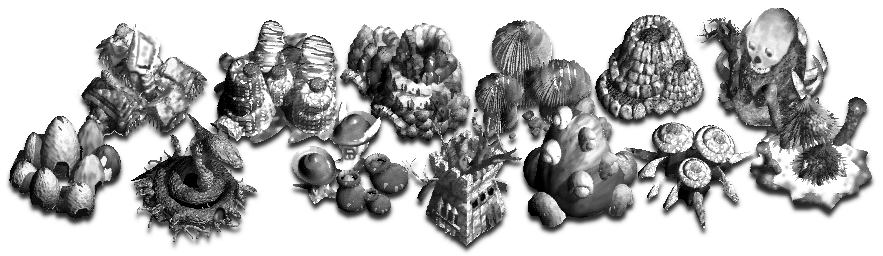
\includegraphics[width=0.7\linewidth]{Ilairs} % Original size?
\end{center}

\textswab{\huge{A}}cross the landscape, you will discover a number of Fryhtan Lairs which harbor beings so horrific as to make any rational description impossible.

If you have set the Fryhtans option to Defensive, these Fryhtans will be of little or no concern if left alone, but once disturbed, they will be a vile and dangerous plague.

If you have set the Fryhtans option to Offensive, they may attack on their own initiative, especially if you build too close to their Lairs.

\section{\textsf{Why Therefore Would You Disturb Them?}}

\index{Fryhtans!disturbing}

You may wish to because throughout the ages they have hoarded vast amounts of wealth as well as the Ancient Scrolls of Power.

You will also notice that when you attack Fryhtans or their Lairs, the Reputation of your Kingdom rises.

Another reason is that in the game’s setup, you may set as your Goal the destruction of all Fryhtans. In this case, it will of course be necessary to attack them.

\section{\textsf{How Do You Relieve Them of Their Wealth?}}

% Ordo is a he.

Every time a Fryhtan Ordo (the Fryhtan equivalent of a General) is slain, he will leave with his bones a pile of gold coins. Send one of your units to this spot, and this treasure will be yours.

\section{\textsf{How Do I Acquire Scrolls of Power?}}

% Ordo is plural? The All High is a he.

Although this is much more difficult, it is also a much greater reward than gold. Scrolls of Power can be acquired by slaying an All High Fryhtan who will issue forth from his Lair only after the dispatch of his Ordo. These Scrolls may only be handled by a unit of the same Nationality as the language of the scroll’s magical inscription.

You will know to which Nationality it belongs by the letter next to each scroll. This will be the first letter of a Nationality. For instance, only a Greek may pick up a Scroll labeled with a G.

\section{\textsf{Of What Use Are the Scrolls of Power?}}

\index{scrolls of power}

The Scrolls of Power grant the mystical knowledge needed to build the Seats of Power and to summon the Greater Beings.

See \textbf{Chapter 16} for details on Seats of Power and Greater Beings.